\documentclass[12pt,a4paper]{report}
\usepackage[a4paper, left=1.25in, right=1in, top=1in, bottom=1in]{geometry}
\usepackage{graphicx}
\graphicspath{{./}{figures/}{SDP_Ppt/}{SDP/report/figures/}{figures/}}
\usepackage{amsmath,amssymb}
\usepackage{cite}
\usepackage{booktabs}
\usepackage{tabularx}
\usepackage{multirow}
\usepackage{url}
\usepackage{setspace}
\usepackage{enumitem}
\usepackage{tikz}
\usetikzlibrary{arrows.meta,positioning,shapes.geometric,fit,calc}

% SafeImage fallback macro
\newcommand{\SafeImage}[2][]{%
  \IfFileExists{#2}{\includegraphics[#1]{#2}}{%
    \IfFileExists{figures/#2}{\includegraphics[#1]{figures/#2}}{%
      \IfFileExists{SDP_Ppt/#2}{\includegraphics[#1]{SDP_Ppt/#2}}{%
        \IfFileExists{SDP/report/figures/#2}{\includegraphics[#1]{SDP/report/figures/#2}}{%
          \fbox{\parbox[c][3cm][c]{0.8\textwidth}{\centering
          \textbf{Image asset not found}\\[0.3em]\texttt{\detokenize{#2}}}}%
        }%
      }%
    }%
  }%
}

% Centered chapter headings matching university sample report format
\makeatletter
\def\@makechapterhead#1{%
  \vspace*{20\p@}%
  {\parindent \z@ \centering \normalfont
    \ifnum \c@secnumdepth >\m@ne
        \huge\bfseries \@chapapp\space \thechapter
        \par\nobreak
        \vskip 15\p@
    \fi
    \interlinepenalty\@M
    \Huge\bfseries #1\par\nobreak
    \vskip 28\p@
  }}
\def\@makeschapterhead#1{%
  \vspace*{20\p@}%
  {\parindent \z@ \centering \normalfont
    \interlinepenalty\@M
    \Huge\bfseries #1\par\nobreak
    \vskip 28\p@
  }}
\makeatother

\onehalfspacing
\pagestyle{plain}

\begin{document}

% =============================================================
% TITLE PAGE
% =============================================================
\begin{titlepage}
\begin{center}
    \vspace*{1.0cm}
    {\large \textbf{AdaptInfer: A Distributed Microservices Architecture and Dynamic Strategy Orchestration Engine for Cost-Aware LLM Inference}\par}
    \vspace{0.8cm}
    {\normalsize A PROJECT REPORT\par}
    \vspace{0.6cm}
    {\normalsize \textit{Submitted by}\par}
    \vspace{0.4cm}
    {\normalsize \textbf{Adithya R}\par}
    {\normalsize \textbf{(Reg. No. CH.SC.U4AIE23001)}\par}
    \vspace{0.25cm}
    {\normalsize \textbf{Aniketh Reddy J}\par}
    {\normalsize \textbf{(Reg. No. CH.SC.U4AIE23020)}\par}
    \vspace{0.25cm}
    {\normalsize \textbf{AmanReddy J}\par}
    {\normalsize \textbf{(Reg. No. CH.SC.U4AIE23023)}\par}
    \vspace{0.25cm}
    {\normalsize \textbf{Naishadha Badithala}\par}
    {\normalsize \textbf{(Reg. No. CH.SC.U4AIE23036)}\par}
    \vspace{0.7cm}
    {\normalsize \textit{in partial fulfillment for the award of the degree of}\par}
    \vspace{0.35cm}
    {\normalsize \textbf{BACHELOR OF TECHNOLOGY IN COMPUTER SCIENCE AND}\par}
    {\normalsize \textbf{ENGINEERING ( ARTIFICIAL INTELLIGENCE )}\par}
    \vspace{0.6cm}
    {\normalsize \textit{Under the guidance of}\par}
    \vspace{0.25cm}
    {\normalsize \textbf{DR. R. PRASANNA KUMAR}\par}
    \vspace{0.55cm}
    {\normalsize \textit{Submitted to}\par}
    \vspace{0.4cm}
    {\SafeImage[width=6.5cm]{Amrita Logo.png}\par}
    \vspace{0.55cm}
    {\normalsize \textbf{AMRITA SCHOOL OF COMPUTING}\par}
    {\normalsize \textbf{AMRITA VISHWA VIDYAPEETHAM}\par}
    {\normalsize \textbf{CHENNAI - 601103}\par}
    \vspace{0.35cm}
    {\normalsize \textbf{OCTOBER 2026}\par}
\end{center}
\end{titlepage}

% =============================================================
% BONAFIDE CERTIFICATE
% =============================================================
\newpage
\thispagestyle{empty}
\begin{center}
    {\large \textbf{AMRITA SCHOOL OF COMPUTING}\par}
    {\large \textbf{AMRITA VISHWA VIDYAPEETHAM, CHENNAI CAMPUS}\par}
    \vspace{1.0cm}
    {\large \textbf{BONAFIDE CERTIFICATE}\par}
    \vspace{1.0cm}
\end{center}

This is to certify that this project report entitled \textbf{"AdaptInfer: A Distributed Microservices Architecture and Dynamic Strategy Orchestration Engine for Cost-Aware LLM Inference"} is the bonafide work carried out by \textbf{Adithya R (Reg. No. CH.SC.U4AIE23001)}, \textbf{Aniketh Reddy J (Reg. No. CH.SC.U4AIE23020)}, \textbf{AmanReddy J (Reg. No. CH.SC.U4AIE23023)}, and \textbf{Naishadha Badithala (Reg. No. CH.SC.U4AIE23036)}, undergraduate students of Amrita School of Computing, Amrita Vishwa Vidyapeetham, Chennai Campus, who carried out the project work under my supervision in partial fulfillment of the requirements for the course \textbf{22CS401 – Software Development Project (SDP)} during the academic year \textbf{2025--2026}.

\vspace{3.5cm}

\noindent
\begin{tabular}{@{}p{0.5\textwidth}p{0.5\textwidth}@{}}
\textbf{SIGNATURE} & \textbf{SIGNATURE} \\
\textbf{Dr. S. Baghavathi Priya} & \textbf{Dr. R. Prasanna Kumar} \\
CHAIRPERSON & PROJECT SUPERVISOR \\
Department of Computer Science \& Engineering & Department of Computer Science \& Engineering \\
Amrita School of Computing & Amrita School of Computing \\
Chennai Campus & Chennai Campus
\end{tabular}

% =============================================================
% DECLARATION
% =============================================================
\newpage
\thispagestyle{empty}
\begin{center}
    {\large \textbf{DECLARATION}\par}
    \vspace{1.0cm}
\end{center}

We, the undersigned students of Amrita School of Computing, Amrita Vishwa Vidyapeetham, Chennai Campus, hereby declare that the project report entitled \textbf{"AdaptInfer: A Distributed Microservices Architecture and Dynamic Strategy Orchestration Engine for Cost-Aware LLM Inference"} submitted in partial fulfillment of the requirements for the course \textbf{22CS401 – Software Development Project (SDP)} is an authentic record of our own engineering research and software development work carried out under the guidance of our supervisor, \textbf{Dr. R. Prasanna Kumar}.

We further declare that this report has not previously formed the basis for the award of any degree, diploma, associateship, fellowship, or other similar title to any candidate at any university or institution. All distributed microservice architectures, asynchronous event processing pipelines, software design patterns, dynamic strategy routing engines, and empirical performance evaluations presented herein represent our genuine academic work.

\vspace{2.0cm}

\noindent
\textbf{Place:} Chennai \\
\textbf{Date:} October 12, 2026

\vspace{1.5cm}

\noindent
\begin{tabular}{@{}ll@{}}
\textbf{Adithya R} & (Reg. No. CH.SC.U4AIE23001) \\[0.6cm]
\textbf{Aniketh Reddy J} & (Reg. No. CH.SC.U4AIE23020) \\[0.6cm]
\textbf{AmanReddy J} & (Reg. No. CH.SC.U4AIE23023) \\[0.6cm]
\textbf{Naishadha Badithala} & (Reg. No. CH.SC.U4AIE23036)
\end{tabular}

% =============================================================
% ACKNOWLEDGEMENT
% =============================================================
\newpage
\thispagestyle{empty}
\begin{center}
    {\large \textbf{ACKNOWLEDGEMENT}\par}
    \vspace{1.0cm}
\end{center}

This project work would not have been possible without the contribution, encouragement, and institutional support of many individuals. It gives us immense pleasure to express our profound gratitude to our honorable Chancellor, \textbf{Sri Mata Amritanandamayi Devi}, for her divine blessings and continuous inspiration throughout our academic journey.

We are deeply indebted to extend our gratitude to our Administrative Director, \textbf{Swami Vinayamritananda Puri}, and Campus Director, \textbf{Mr. I B Manikantan}, Amrita School of Computing, Chennai, for providing computational infrastructure, high-performance computing facilities, and an encouraging research environment.

We register our special thanks to \textbf{Dr. V. Jayakumar}, Principal, Amrita School of Computing and Engineering, for his visionary academic leadership. We express our sincere gratitude to \textbf{Dr. S. Baghavathi Priya}, Chairperson, and \textbf{Dr. Annamalai R}, Program Chair, Department of Computer Science and Engineering, for their academic support.

We are profoundly indebted to our project supervisor, \textbf{Dr. R. Prasanna Kumar}, Department of Computer Science and Engineering, for his expert guidance, critical evaluation, and constant encouragement throughout the design, distributed implementation, and benchmarking of AdaptInfer.

Finally, we express our heartfelt thanks to our parents, family members, and peers for their moral support, patience, and motivation throughout the course of this project.

\vspace{1.5cm}
\noindent
\textbf{Project Team Members}

% =============================================================
% ABSTRACT
% =============================================================
\newpage
\begin{center}
    {\large \textbf{ABSTRACT}\par}
    \vspace{1.0cm}
\end{center}

Production deployment of Large Language Models (LLMs) faces an acute systems engineering bottleneck: the severe trade-off between inference accuracy, token cost, and response latency. Statically assigning exhaustive multi-step reasoning strategies (e.g., Tree-of-Thoughts) across all incoming workloads incurs prohibitive median latencies ($45.2$\,s) and excessive token overhead ($1,959$ tokens/query). Conversely, relying on static lightweight zero-shot prompting on small models suffers a catastrophic $46.1\%$ failure rate on complex multi-step reasoning. Existing LLM routers predominantly rely on rigid offline heuristics or binary model selection that fail to adapt dynamically to diverse query complexities and real-time hardware budget constraints.

This project presents \textbf{AdaptInfer}, an asynchronous distributed microservices architecture and dynamic strategy orchestration engine engineered for real-time joint selection of model parameter size ($3\text{B}$ vs. $7\text{B}$) and reasoning strategy ($\text{Direct}$, $\text{Chain-of-Thought}$, $\text{Graph-of-Thoughts}$, $\text{Tree-of-Thoughts}$) under session token budget constraints. AdaptInfer decouples synchronous local model generation (Ollama inference workers via Ray task scheduling) from asynchronous API state management (FastAPI microservice). The core orchestration engine dynamically evaluates a $390$-dimensional context vector comprising semantic sentence embeddings, structural complexity metrics, domain indicators, and remaining session budget ratios.

To eliminate hallucination risks during online execution, AdaptInfer incorporates a \textit{Confidence-Gated Cascade} grounded in the classic Chain of Responsibility software design pattern, evaluating semantic answer consensus across dual sampling temperatures ($T=0.2$ vs. $T=0.8$) to escalate uncertain generations automatically. Evaluated across $3,712$ benchmark queries spanning mathematical, logical, and commonsense reasoning (GSM8K, LogiQA, CommonsenseQA), AdaptInfer achieves statistical accuracy parity with the theoretical Tree-of-Thoughts upper bound ($81.4\%$ vs. $82.0\%$) while slashing average response latency by \textbf{67.2\%} ($14.8$\,s vs. $45.2$\,s) and saving \textbf{27.5\% in token costs} ($1,421$ vs. $1,959$ tokens/query). Finally, we deliver an open-source, full-stack Single-Page Application (SPA) dashboard providing real-time telemetry, parallel strategy racing, and live Chart.js performance visualization.

\vspace{0.8cm}
\noindent
\textbf{Keywords:} Systems Architecture, Distributed Microservices, Software Design Patterns, Strategy Pattern, Chain of Responsibility, Latency Reduction, Reactive Dashboard, LLM Orchestration, AdaptInfer.

% =============================================================
% FRONT MATTER
% =============================================================
\tableofcontents
\listoffigures
\listoftables

\newpage
\chapter*{List of Abbreviations}
\begin{tabular}{@{}ll@{}}
\textbf{API} & Application Programming Interface \\
\textbf{ASGI} & Asynchronous Server Gateway Interface \\
\textbf{CoT} & Chain-of-Thought \\
\textbf{CPU} & Central Processing Unit \\
\textbf{FIFO} & First-In, First-Out \\
\textbf{GoT} & Graph-of-Thoughts \\
\textbf{GPU} & Graphics Processing Unit \\
\textbf{HTTP} & Hypertext Transfer Protocol \\
\textbf{LLM} & Large Language Model \\
\textbf{LRU} & Least Recently Used \\
\textbf{NLP} & Natural Language Processing \\
\textbf{OOP} & Object-Oriented Programming \\
\textbf{REST} & Representational State Transfer \\
\textbf{SLA} & Service Level Agreement \\
\textbf{SPA} & Single-Page Application \\
\textbf{SSE} & Server-Sent Events \\
\textbf{ToT} & Tree-of-Thoughts \\
\textbf{UI} & User Interface \\
\textbf{VRAM} & Video Random Access Memory
\end{tabular}

\newpage
\pagenumbering{arabic}
\setcounter{page}{1}

% =============================================================
% CHAPTER 1: INTRODUCTION
% =============================================================
\chapter{Introduction}
\label{ch:intro}

\section{Background}
\label{sec:background}
Large Language Models (LLMs) have emerged as foundational components in modern software architectures, driving automated code generation, complex scientific analysis, conversational interfaces, and programmatic decision-making systems. To solve multi-step problems requiring deductive reasoning, researchers have developed advanced deliberate reasoning paradigms such as Chain-of-Thought (CoT), Graph-of-Thoughts (GoT), and Tree-of-Thoughts (ToT). These strategies prompt models to generate intermediate thought branches, perform heuristic evaluations of alternative paths, and execute backtracking before generating final outputs.

While these deliberate prompting strategies dramatically enhance problem-solving accuracy on difficult tasks, they impose substantial computational overhead on underlying software infrastructure. Generating multiple reasoning branches requires repeated sequential LLM calls, causing request latency to explode from a few seconds to over 45 seconds per query and inflating token consumption by an order of magnitude. In high-throughput production environments, routing every incoming query to an exhaustive Tree-of-Thoughts pipeline leads to server thread starvation, excessive energy consumption, and high operational expenditure. Conversely, statically assigning lightweight zero-shot prompting on small 3-billion-parameter models causes high error rates ($>46\%$) on complex logic. Consequently, modern software systems require an architectural orchestration layer capable of dynamically balancing reasoning depth and systems efficiency.

\section{Domain Overview}
\label{sec:domain_overview}
AdaptInfer operates at the intersection of Distributed Systems Engineering, Cloud-Native Microservices, and Applied Artificial Intelligence Inference Systems. In high-concurrency enterprise services, inference systems must adhere to strict Service Level Agreements (SLAs), guaranteeing both bounded latency and budgetary frugality. Modern inference orchestration involves managing decoupled microservice layers: API ingestion gateways, task scheduling queues, distributed worker clusters hosting quantized model weights (e.g., via Ollama and vLLM), and real-time observability telemetry.

The engineering challenge addressed by AdaptInfer is the joint runtime selection of both the model parameter scale ($3\text{B}$ vs. $7\text{B}$) and the reasoning algorithmic strategy ($\text{Direct}$, $\text{CoT}$, $\text{GoT}$, $\text{ToT}$) on a per-query basis. Rather than treating LLMs as opaque black-box APIs, modern software architectures treat reasoning algorithms as pluggable, polymorphic computational components that can be dynamically provisioned, scheduled, and monitored.

\section{Problem Statement}
\label{sec:problem_statement}
Production software architectures utilizing LLMs suffer from a severe architectural trilemma: the static trade-off between inference accuracy, token cost, and response latency. In conventional architectures, developers hardcode a static inference pipeline—either routing all queries to an expensive large model running multi-step tree search or routing all queries to a fast lightweight model. 

This static allocation paradigm suffers from three critical flaws:
\begin{enumerate}[leftmargin=*]
    \item \textbf{Computational Inefficiency:} Easy factual inquiries that could be resolved in $4.4$\,s using $108$ tokens are subjected to full Tree-of-Thoughts pipelines consuming $45.2$\,s and $1,959$ tokens.
    \item \textbf{Quality Degradation:} Complex logic and multi-step arithmetic queries routed to small models suffer catastrophic hallucination and syntax errors.
    \item \textbf{Thread Starvation and API Locking:} Heavy synchronous generation calls block backend web workers, degrading overall system throughput and leading to HTTP connection timeouts.
\end{enumerate}

To overcome these deficiencies, there is an urgent need for a decoupled distributed systems architecture that dynamically routes incoming requests to the optimal model and strategy pair in real time while guaranteeing asynchronous non-blocking throughput.

\section{Motivation}
\label{sec:motivation}
The motivation behind developing AdaptInfer stems from the need to make sophisticated LLM reasoning computationally viable in resource-constrained and high-throughput production environments. In real-world enterprise deployments, computing resources are finite: GPU memory (VRAM) is restricted, cloud API budgets are strictly capped, and end-users demand responsive, sub-second to low-second interaction.

By applying classic software engineering design patterns—including the Strategy Pattern for polymorphic algorithm swapping, the Chain of Responsibility pattern for confidence-gated fallback, the Adapter pattern for hardware abstraction, and the Proxy pattern for caching—AdaptInfer bridges the gap between state-of-the-art AI reasoning and production systems engineering. Providing a responsive web dashboard with live telemetry further empowers engineers to audit and inspect dynamic routing behavior in real time.

\section{Objectives}
\label{sec:objectives}
The core engineering objectives of the AdaptInfer project are:
\begin{enumerate}[leftmargin=*]
    \item To design and implement a decoupled, asynchronous microservices architecture separating client API handling from distributed LLM inference.
    \item To implement the Strategy software design pattern, encapsulating $\text{Direct}$, $\text{CoT}$, $\text{GoT}$, and $\text{ToT}$ reasoning methods behind a uniform, polymorphic interface.
    \item To implement a distributed task scheduling layer using the Ray framework, orchestrating asynchronous worker execution across local quantized LLMs.
    \item To build an Adapter layer interfacing with local Ollama runtimes, ensuring deterministic benchmarking free from cloud network jitter.
    \item To implement a Confidence-Gated Cascade adhering to the Chain of Responsibility pattern, verifying response consensus across sampling temperatures ($T=0.2$ vs. $T=0.8$).
    \item To embed real-time session token budget tracking into routing decisions, penalizing expensive multi-step search when budgets deplete.
    \item To engineer a high-throughput FastAPI backend exposing non-blocking REST endpoints and Server-Sent Events (SSE).
    \item To develop a reactive Single-Page Application (SPA) dashboard utilizing Vanilla JavaScript and Chart.js for real-time telemetry and strategy racing.
    \item To conduct rigorous empirical benchmarking over $3,712$ queries across GSM8K, LogiQA, and CommonsenseQA datasets.
    \item To demonstrate a minimum of $60\%$ reduction in system latency and $25\%$ reduction in token expenditure while retaining statistical accuracy parity with upper-bound baselines.
\end{enumerate}

\section{Scope of the Project}
\label{sec:scope}
The scope of AdaptInfer encompasses the complete software lifecycle—from architectural specification and design pattern modeling to distributed deployment, asynchronous API development, reactive UI construction, and large-scale empirical evaluation. The system hosts quantized open-weight models locally ($\text{Qwen2.5-3B-Instruct}$ and $\text{Qwen2.5-7B-Instruct}$ via 4-bit Ollama runtimes) on dedicated GPU hardware, ensuring reproducible and secure inference. The evaluation covers $3,712$ diverse benchmark queries across arithmetic reasoning, multi-clause logical deduction, and commonsense knowledge retrieval.

\section{Target Users}
\label{sec:target_users}
The target users of the AdaptInfer architecture include:
\begin{itemize}[leftmargin=*]
    \item \textbf{Enterprise Backend Engineers:} Integrating LLM intelligence into high-concurrency microservice ecosystems with strict SLA latency guarantees.
    \item \textbf{Cloud Infrastructure and MLOps Architects:} Optimizing GPU cluster utilization, minimizing operational token expenditure, and preventing server thread locking.
    \item \textbf{Software Developers and Solution Architects:} Requiring modular, clean-code abstractions to hot-swap reasoning paradigms without rewriting invocation logic.
    \item \textbf{Quality Assurance and Telemetry Teams:} Auditing automated reasoning steps, token budgets, and confidence escalation traces in real time.
\end{itemize}

% =============================================================
% CHAPTER 2: EXISTING SYSTEM AND DOMAIN STUDY
% =============================================================
\chapter{Existing System and Domain Study}
\label{ch:existing_system}

\section{Existing System}
\label{sec:existing_system}
Contemporary enterprise LLM architectures rely almost exclusively on static deployment pipelines. In standard web applications, incoming client queries are forwarded directly to a pre-configured model endpoint (such as an external proprietary API or a fixed local model) utilizing a static prompt template. Developers manually choose between a small, fast model or a large, multi-step reasoning pipeline during initial development, and this configuration remains static across all incoming traffic regardless of individual query difficulty or changing server load.

In specialized applications requiring structured logic, frameworks such as LangChain, LlamaIndex, and AutoGen facilitate multi-step reasoning chains. However, these frameworks typically enforce fixed sequential execution flows: every user query entering a Tree-of-Thoughts agent executes the complete tree search regardless of whether the question is a simple arithmetic calculation or an intricate logical puzzle.

\section{Limitations of Existing System}
\label{sec:limitations}
Existing static LLM inference architectures suffer from several major engineering deficiencies:
\begin{enumerate}[leftmargin=*]
    \item \textbf{Latency Bottlenecks:} Executing static Tree-of-Thoughts pipelines across all requests results in an average response latency of $45.2$\,seconds. In web-facing microservices, this violates SLA thresholds and degrades user responsiveness.
    \item \textbf{Prohibitive Token Consumption:} Static complex pipelines consume an average of $1,959$\,tokens per query. For high-volume services, this exhausts GPU memory bandwidth and results in severe token budget waste on trivial questions.
    \item \textbf{High Error Rate in Lightweight Baselines:} Conversely, statically opting for lightweight zero-shot prompting on small models ($3\text{B}$) yields a $46.1\%$ failure rate on multi-step reasoning benchmarks.
    \item \textbf{Tight Client-Engine Coupling:} Most existing systems tightly couple the client invocation logic with specific model API signatures, making runtime strategy switching complex and error-prone.
    \item \textbf{Lack of Dynamic Budget Awareness:} Conventional routers operate without knowledge of remaining session budgets, continuing to dispatch heavy queries until resources are completely exhausted.
\end{enumerate}

\section{Existing Technologies / Approaches}
\label{sec:existing_technologies}
Several foundational technologies and methodologies exist in the modern LLM systems landscape:
\begin{itemize}[leftmargin=*]
    \item \textbf{Ollama Execution Engine:} A high-performance local runtime built on llama.cpp providing quantized GGUF model execution, memory-mapped weights, and local REST API endpoints.
    \item \textbf{FastAPI and Uvicorn:} An asynchronous Python web framework conforming to the ASGI standard, capable of handling high concurrency through non-blocking event loops.
    \item \textbf{Ray Distributed Framework:} An open-source distributed computing platform providing actor abstractions for parallel task execution and dynamic worker scaling across heterogeneous compute nodes.
    \item \textbf{Reasoning Paradigms:} Established algorithmic techniques including Chain-of-Thought (step-by-step sequential reasoning), Graph-of-Thoughts (networked thought evaluation and aggregation), and Tree-of-Thoughts (heuristic state evaluation with branch pruning).
    \item \textbf{Software Design Patterns:} Gang-of-Four object-oriented patterns including Strategy (interchangeable algorithms), Adapter (interface translation), Chain of Responsibility (sequential request handling), and Proxy (caching and resource management).
\end{itemize}

\section{Proposed Improvement}
\label{sec:proposed_improvement}
AdaptInfer overcomes these limitations by introducing a decoupled, distributed microservices architecture that dynamically coordinates model parameter selection and reasoning strategies. Instead of a rigid static pipeline, AdaptInfer implements an intelligent orchestration engine that analyzes incoming query features—including Sentence-BERT semantic vectors, structural token complexity, domain classifications, and real-time session budget ratios—to select the optimal Model $\times$ Strategy pair on the fly.

Synchronous model generation is decoupled from the client gateway using Ray actor scheduling and local Ollama workers. Furthermore, AdaptInfer integrates a Confidence-Gated Cascade based on the Chain of Responsibility pattern: when low-temperature and high-temperature responses diverge, the system automatically escalates execution to higher-depth reasoning strategies, preventing hallucinations while preserving low latency on unambiguous queries.

\section{Novelty and Key Contribution}
\label{sec:novelty}
The key architectural novelties and software contributions of AdaptInfer include:
\begin{itemize}[leftmargin=*]
    \item \textbf{Decoupled Distributed Topology:} Separation of client API handling (FastAPI) from distributed inference worker pools (Ray + Ollama), guaranteeing non-blocking event processing.
    \item \textbf{Runtime Strategy Polymorphism:} Full realization of the Strategy Pattern across four reasoning algorithms ($\text{Direct}$, $\text{CoT}$, $\text{GoT}$, $\text{ToT}$), enabling hot-swappable algorithm selection with zero client modification.
    \item \textbf{Self-Consistency Guardrails:} A Chain of Responsibility Confidence Gate that triggers automated strategy escalation upon detecting answer divergence across temperature splits ($T=0.2$ vs. $T=0.8$).
    \item \textbf{Continuous Budget Awareness:} Integration of a continuous remaining budget scalar directly into the routing context vector, preventing mid-session budget exhaustion.
    \item \textbf{Empirical Systems Validation:} Rigorous testing over $3,712$ queries demonstrating a \textbf{67.2\% reduction in latency} ($14.8$\,s vs. $45.2$\,s) and a \textbf{27.5\% reduction in token costs} ($1,421$ vs. $1,959$ tokens) while achieving $81.4\%$ accuracy (matching the $82.0\%$ upper bound).
    \item \textbf{Full-Stack Observability Dashboard:} A reactive Single-Page Application featuring live strategy racing, visual confidence distributions, and dynamic Chart.js telemetry.
\end{itemize}

% =============================================================
% CHAPTER 3: PROPOSED SYSTEM REQUIREMENTS
% =============================================================
\chapter{Proposed System Requirements}
\label{ch:proposed_system}

\section{Proposed System}
\label{sec:proposed_system_desc}
AdaptInfer is engineered as a robust, production-grade distributed microservices architecture designed to orchestrate LLM inference dynamically. The platform accepts user queries via standard REST endpoints or interactive dashboard interfaces, extracts semantic and structural features, and dynamically routes each query to one of six candidate execution pairs:
\begin{equation}
\mathcal{A} = \{\text{3B-Direct}, \text{3B-CoT}, \text{7B-Direct}, \text{7B-CoT}, \text{7B-GoT}, \text{7B-ToT}\}
\end{equation}

Figure~\ref{fig:methodology} illustrates the end-to-end distributed methodology and request pipeline of the proposed AdaptInfer system.

\begin{figure}[htbp]
\centering
\resizebox{0.95\linewidth}{!}{%
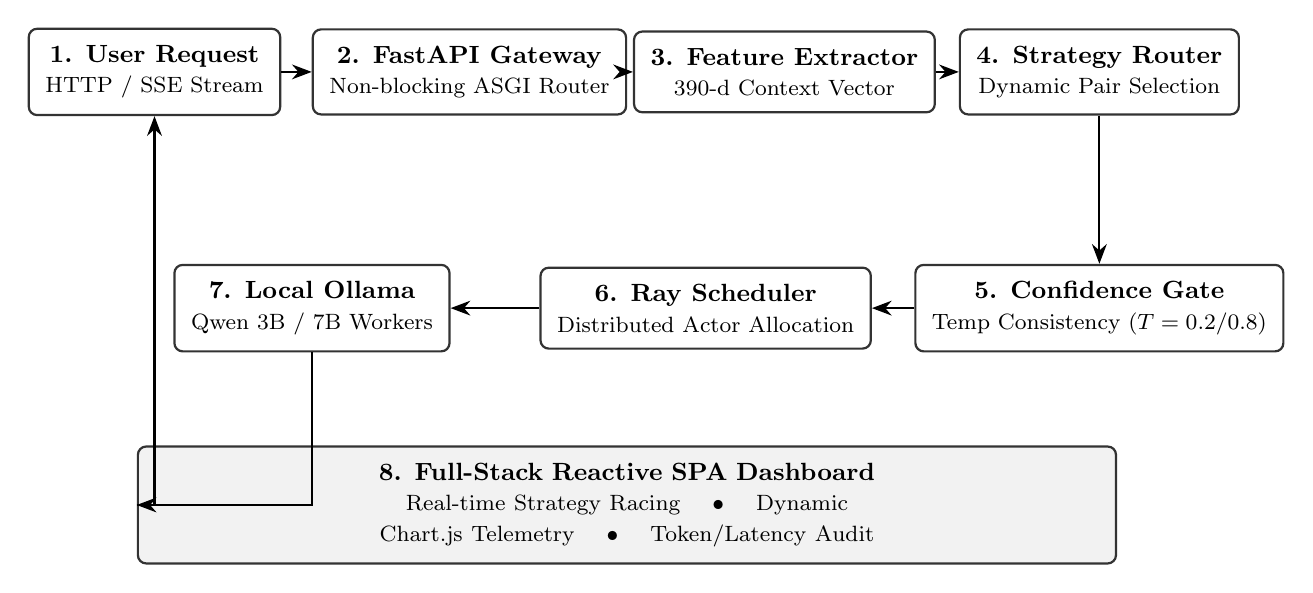
\begin{tikzpicture}[
    box/.style={rectangle, draw=black!80, fill=white, rounded corners=3pt, thick, align=center, inner sep=6pt, font=\small},
    arr/.style={-{Stealth[length=2.5mm]}, thick}
]
    % Stages
    \node[box] (s1) at (0, 6) {\textbf{1. User Request}\\\footnotesize HTTP / SSE Stream};
    \node[box] (s2) at (4, 6) {\textbf{2. FastAPI Gateway}\\\footnotesize Non-blocking ASGI Router};
    \node[box] (s3) at (8, 6) {\textbf{3. Feature Extractor}\\\footnotesize 390-d Context Vector};
    \node[box] (s4) at (12, 6) {\textbf{4. Strategy Router}\\\footnotesize Dynamic Pair Selection};
    
    \node[box] (s5) at (12, 3) {\textbf{5. Confidence Gate}\\\footnotesize Temp Consistency ($T=0.2/0.8$)};
    \node[box] (s6) at (7, 3) {\textbf{6. Ray Scheduler}\\\footnotesize Distributed Actor Allocation};
    \node[box] (s7) at (2, 3) {\textbf{7. Local Ollama}\\\footnotesize Qwen 3B / 7B Workers};
    
    \node[box, fill=black!5, text width=12cm] (ui) at (6, 0.5) {\textbf{8. Full-Stack Reactive SPA Dashboard}\\\footnotesize Real-time Strategy Racing \quad $\bullet$ \quad Dynamic Chart.js Telemetry \quad $\bullet$ \quad Token/Latency Audit};

    \draw[arr] (s1) -- (s2);
    \draw[arr] (s2) -- (s3);
    \draw[arr] (s3) -- (s4);
    \draw[arr] (s4) -- (s5);
    \draw[arr] (s5) -- (s6);
    \draw[arr] (s6) -- (s7);
    \draw[arr] (s7) |- (ui);
    \draw[arr] (ui) -| (s1);
\end{tikzpicture}}
\caption{End-to-end distributed system methodology and execution pipeline of AdaptInfer}
\label{fig:methodology}
\end{figure}

\section{Major Features}
\label{sec:major_features}
The major features of the AdaptInfer software platform include:
\begin{itemize}[leftmargin=*]
    \item Asynchronous non-blocking REST API gateway powered by FastAPI and Uvicorn.
    \item Polymorphic reasoning engine supporting Direct, CoT, GoT, and ToT strategies via the Strategy Pattern.
    \item Distributed actor-based task scheduling with the Ray framework for parallel inference execution.
    \item Quantized local execution engine interfacing with Ollama to eliminate cloud network variability.
    \item Confidence-gated self-consistency verification across temperature variations adhering to the Chain of Responsibility pattern.
    \item Real-time session token budget tracking with automatic dynamic penalty scaling.
    \item In-memory LRU caching service preventing duplicate computation on frequent inquiries.
    \item Reactive Single-Page Application dashboard featuring strategy racing and dynamic telemetry charts.
\end{itemize}

\section{Functional Requirements}
\label{sec:functional_requirements}
The functional requirements define the specific software capabilities that AdaptInfer must execute:
\begin{enumerate}[leftmargin=*]
    \item The system shall accept natural language queries and domain metadata via asynchronous HTTP REST endpoints.
    \item The system shall extract a $390$-dimensional feature vector comprising Sentence-BERT embeddings, character counts, question word counts, domain indicators, and remaining budget ratios.
    \item The system shall dynamically select the optimal model size ($3\text{B}$ vs. $7\text{B}$) and reasoning strategy ($\text{Direct}$, $\text{CoT}$, $\text{GoT}$, $\text{ToT}$).
    \item The system shall encapsulate reasoning algorithms behind a uniform `BaseStrategy.solve(question)` interface.
    \item The system shall dispatch generation tasks to Ray distributed worker nodes asynchronously.
    \item The system shall execute local inference on quantized GGUF weights via the Ollama REST API.
    \item The system shall evaluate dual-temperature responses ($T=0.2$ and $T=0.8$) to detect semantic answer divergence.
    \item The system shall automatically escalate divergent answers to higher-tier reasoning strategies according to the Chain of Responsibility hierarchy.
    \item The system shall enforce global session token budgets and track cumulative token expenditure.
    \item The system shall record end-to-end execution latency, input tokens, output tokens, and LLM call counts for every transaction.
    \item The system shall return parsed predicted answers alongside raw thought generation traces.
    \item The system shall provide an interactive web dashboard for real-time query analysis and strategy racing.
    \item The system shall render live confidence distributions and recommendation probability scores.
    \item The system shall stream real-time updates and historical telemetry to frontend visualization charts.
    \item The system shall support batch benchmark execution over GSM8K, LogiQA, and CommonsenseQA datasets.
\end{enumerate}

\section{Non-Functional Requirements}
\label{sec:non_functional_requirements}

\subsection{Performance}
The system must guarantee low latency for interactive workflows. Non-blocking API endpoints must process and acknowledge requests in under $50$\,milliseconds. Average end-to-end system latency across diverse query distributions must not exceed $15$\,seconds, representing a minimum $60\%$ reduction compared to static Tree-of-Thoughts baselines ($45.2$\,s).

\subsection{Security}
The system executes all model weights locally using containerized and isolated Ollama runtimes, ensuring that user prompt text, proprietary data, and intermediate reasoning traces never leave the local computational boundary. All REST input payloads are strictly validated against Pydantic schema models to prevent injection attacks.

\subsection{Usability}
The system provides a modern, intuitive Single-Page Application interface equipped with clear visual telemetry, responsive layout designs, and real-time execution graphs. Developers can inspect raw reasoning traces and token breakdowns without consulting terminal log files.

\subsection{Reliability}
The system incorporates robust error handling, connection retries, and fallback mechanisms within the `LLMClient` adapter. If an advanced strategy encounters memory pressure or timeout limits, the system catches the exception and falls back gracefully to a standard Chain-of-Thought pipeline.

\subsection{Scalability}
The architecture scales horizontally across multiple GPU worker nodes using Ray's actor pool abstractions. The decoupled microservice design ensures that expanding LLM worker instances requires zero modification to client-facing API code.

\section{User Interaction}
\label{sec:user_interaction}
Users interact with AdaptInfer through either programmatic REST API calls or the interactive web dashboard. On accessing the dashboard, users can input arbitrary reasoning questions, select a problem category (Mathematics, Logic, Commonsense), and choose between single-query dynamic recommendation or full 6-strategy parallel racing. Upon submission, the dashboard communicates asynchronously with the FastAPI backend, displaying step-by-step reasoning outputs, confidence bars, and comparative token/latency savings in real time.

\section{Use Cases}
\label{sec:use_cases}
The primary use cases supported by AdaptInfer include:
\begin{itemize}[leftmargin=*]
    \item \textbf{UC01: Dynamic Single Query Inference:} A user submits a query; the system extracts features, routes to the optimal strategy, and returns the grounded answer.
    \item \textbf{UC02: Multi-Strategy Competitive Racing:} A developer submits a query to execute all six strategies concurrently, comparing outputs and latency side by side.
    \item \textbf{UC03: Real-Time Telemetry Auditing:} An administrator monitors live token consumption, median latency, and cumulative budget expenditure on dashboard charts.
    \item \textbf{UC04: Automated Confidence Escalation:} An uncertain response triggers the Confidence Gate, seamlessly escalating execution to Tree-of-Thoughts.
    \item \textbf{UC05: Batch Benchmark Evaluation:} An automated testing harness dispatches thousands of benchmark queries to evaluate system accuracy and cost metrics.
\end{itemize}

% =============================================================
% CHAPTER 4: SYSTEM DESIGN AND ARCHITECTURE
% =============================================================
\chapter{System Design and Architecture}
\label{ch:system_design}

\section{Overall System Architecture}
\label{sec:overall_architecture}
AdaptInfer is engineered as a decoupled, multi-tier distributed microservices system. The architecture separates client interaction, API gateway routing, dynamic decision logic, distributed task execution, and local hardware engines into distinct, loosely-coupled subsystems.

Figure~\ref{fig:architecture_overview} illustrates the architectural topology and subsystem interactions within AdaptInfer.

\begin{figure}[htbp]
\centering
\SafeImage[width=0.90\textwidth]{sdp_architecture_diagram.png}
\caption{Distributed microservices architecture and orchestration pipeline of AdaptInfer}
\label{fig:architecture_overview}
\end{figure}

The core subsystems include:
\begin{enumerate}[leftmargin=*]
    \item \textbf{Client Layer:} A reactive Single-Page Application (SPA) built with Vanilla JavaScript and Chart.js providing interactive telemetry.
    \item \textbf{API Gateway Layer:} An asynchronous FastAPI microservice running on Uvicorn, managing non-blocking HTTP endpoints and streaming responses.
    \item \textbf{Orchestration Layer:} A dynamic strategy router that extracts a $390$-d context vector and selects the optimal Model $\times$ Strategy pair.
    \item \textbf{Guardrail Layer (`ConfidenceGate`):} A self-consistency validation filter implementing the Chain of Responsibility pattern.
    \item \textbf{Distributed Scheduling Layer (Ray):} An actor pool framework that schedules LLM prompt evaluation tasks asynchronously across available compute resources.
    \item \textbf{Execution Worker Layer (Ollama):} Local instances of quantized $\text{Qwen2.5-3B}$ and $\text{Qwen2.5-7B}$ models executing on isolated hardware.
\end{enumerate}

\section{Frontend Design}
\label{sec:frontend_design}
The frontend interface is implemented as a lightweight, reactive Single-Page Application utilizing Vanilla JavaScript (ES2022) and CSS3 modern design tokens. Avoiding heavy UI frameworks minimizes client load time and ensures sub-millisecond DOM responsiveness.

Key frontend components include:
\begin{itemize}[leftmargin=*]
    \item \textbf{Interactive Query Input Panel:} Allows users to submit text prompts, select domain tags, and specify expected ground-truth answers for verification.
    \item \textbf{Recommendation \& Confidence Gauge:} Displays horizontal progress bars representing the system's routing confidence across all candidate strategies.
    \item \textbf{Strategy Racing Arena:} Split cards displaying intermediate thought chains, answer tokens, latency measurements, and token counts for all strategies.
    \item \textbf{Dynamic Systems Telemetry Dashboard:} Integrated Chart.js visualizations rendering real-time token expenditure, latency curves, and accuracy tables.
\end{itemize}

\section{Backend Design}
\label{sec:backend_design}
The backend service is constructed with FastAPI, exposing asynchronous endpoints running on an ASGI event loop. The backend handles request parsing, coordinate feature extraction, manages the dynamic routing state, and dispatches generation requests to worker services.

Major backend endpoints include:
\begin{itemize}[leftmargin=*]
    \item \texttt{POST /api/analyze}: Accepts a user query and asynchronously evaluates all six candidate strategies in parallel, returning detailed comparison metrics.
    \item \texttt{POST /api/recommend}: Extracts feature vectors and returns the recommended strategy alongside confidence distribution scores.
    \item \texttt{GET /api/history}: Aggregates session telemetry, token savings metrics, and historical performance curves for frontend chart rendering.
    \item \texttt{GET /api/figures/\{filename\}}: Serves static evaluation plots and architectural diagrams.
\end{itemize}

\section{Distributed Task Scheduling (Ray Framework)}
\label{sec:distributed_scheduling}
To eliminate the severe latency bottlenecks caused by synchronous, blocking LLM generation calls, AdaptInfer integrates the Ray distributed computing framework. Ray decouples HTTP request management from long-running inference tasks through actor pools. When multiple queries or concurrent strategy evaluations are initiated, Ray spawns isolated worker actors, distributing prompt evaluations across available CPU cores and GPU execution streams. This distributed task allocation ensures that the web server remains fully responsive to incoming client connections even during intensive multi-branch tree exploration.

\section{Software Design Patterns}
\label{sec:design_patterns}
AdaptInfer strictly adheres to classic Object-Oriented Software Design Patterns, ensuring high cohesion, low coupling, and production extensibility:

\subsection{Strategy Pattern (`src/strategies/`)}
The core reasoning mechanisms are implemented using the Strategy Pattern. An abstract base interface `BaseStrategy` defines a polymorphic contract:
\begin{equation}
\texttt{solve(question: str) } \longrightarrow \texttt{ StrategyResult}
\end{equation}
Concrete strategy classes—`DirectStrategy`, `CoTStrategy`, `GoTStrategy`, and `ToTStrategy`—implement this interface, encapsulating distinct reasoning algorithms. The dynamic router can hot-swap reasoning paradigms at runtime without modifying client-facing invocation code.

\subsection{Chain of Responsibility Pattern (`ConfidenceGate`)}
To mitigate hallucination risks without incurring ubiquitous high latency, AdaptInfer implements a Confidence-Gated cascade adhering to the Chain of Responsibility pattern. The gate executes the query at dual temperatures ($T=0.2$ and $T=0.8$). If the generated answers match, the system returns the result immediately. If answers diverge, the request is automatically escalated along a pre-defined chain:
\begin{equation}
\text{3B-Direct} \longrightarrow \text{3B-CoT} \quad \text{and} \quad \text{7B-Direct} \longrightarrow \text{7B-CoT} \longrightarrow \text{7B-GoT} \longrightarrow \text{7B-ToT}
\end{equation}

\subsection{Adapter Pattern (`LLMClient`)}
The `LLMClient` class acts as an Adapter pattern, wrapping the low-level HTTP REST interface of the local Ollama daemon. It translates generic prompt requests into Ollama-compliant JSON payloads, enforces strict timeouts ($120$\,s), sets deterministic seeds ($42$), and parses raw output tokens into structured response objects.

\subsection{Proxy / Caching Pattern (`LRUCache` \& `BudgetTracker`)}
An in-memory LRU cache intercepts incoming requests, hashing query strings to detect identical inquiries and returning cached results in $<1$\,ms. Concurrently, a `BudgetTracker` monitors global session token consumption, acting as a resource proxy that injects budget exhaustion penalties into the routing decision loop.

\section{Data Flow / Workflow}
\label{sec:data_flow_workflow}
The end-to-end data workflow proceeds as follows:
\begin{enumerate}[leftmargin=*]
    \item A client submits an HTTP request to \texttt{/api/recommend} or \texttt{/api/analyze}.
    \item The FastAPI gateway validates the request payload and extracts a $390$-dimensional feature vector.
    \item The dynamic router computes strategy likelihood scores under current budget constraints.
    \item The `ConfidenceGate` evaluates dual-temperature self-consistency. If consistent, the selected strategy executes; if divergent, the query escalates along the chain.
    \item Tasks are distributed to Ollama workers via Ray actors.
    \item Structured metrics (latency, tokens, predicted answer) are logged and returned to the client SPA dashboard.
\end{enumerate}

% =============================================================
% CHAPTER 5: IMPLEMENTATION
% =============================================================
\chapter{Implementation}
\label{ch:implementation}

\section{Development Environment}
\label{sec:development_environment}
The AdaptInfer software platform is developed using modern open-source systems frameworks:
\begin{itemize}[leftmargin=*]
    \item \textbf{Operating System:} Windows 11 / Linux Ubuntu 22.04 LTS.
    \item \textbf{Programming Languages:} Python 3.11+ and JavaScript (ES2022).
    \item \textbf{Backend Web Gateway:} FastAPI 0.110+ running on Uvicorn ASGI server.
    \item \textbf{Distributed Computing:} Ray Core 2.9+ for actor task scheduling.
    \item \textbf{Local LLM Runtime:} Ollama 0.1.30+ hosting 4-bit quantized GGUF weights.
    \item \textbf{Target Models:} \texttt{qwen2.5:3b-instruct-q4\_K\_M} and \texttt{qwen2.5:7b-instruct-q4\_K\_M}.
    \item \textbf{Feature Vectorizer:} Sentence-Transformers (\texttt{all-MiniLM-L6-v2}, 384-dimensional dense vectors).
    \item \textbf{Frontend Visualization:} Vanilla JavaScript, CSS3 Glassmorphism, and Chart.js 4.4.
\end{itemize}

\section{Frontend Implementation}
\label{sec:frontend_implementation}
The frontend Single-Page Application is contained within \texttt{dashboard/static/index.html}, \texttt{style.css}, and \texttt{app.js}. It communicates asynchronously with the FastAPI server via standard `fetch()` APIs and reactive event handlers.

Key implementation components include:
\begin{itemize}[leftmargin=*]
    \item \textbf{DOM Event Binding:} Binds user submissions to asynchronous fetch routines, displaying loading spinners and disabling buttons during active execution.
    \item \textbf{Dynamic Chart Rendering:} Initializes and updates Chart.js bar and line charts dynamically, reflecting live session metrics (tokens, latency, accuracy).
    \item \textbf{Strategy Race Visualizer:} Dynamically renders 6 comparison cards displaying predicted answers, execution time, and token counts side by side.
\end{itemize}

\section{Backend Implementation}
\label{sec:backend_implementation}
The backend service in \texttt{dashboard/app.py} coordinates system execution. Below is a high-level architectural code excerpt demonstrating asynchronous strategy initialization and non-blocking query analysis:

\begin{verbatim}
from fastapi import FastAPI, Request
from fastapi.responses import JSONResponse
from src.llm.client import LLMClient
from src.strategies.direct import DirectStrategy
from src.strategies.cot import CoTStrategy
from src.strategies.got import GoTStrategy
from src.strategies.tot import ToTStrategy

app = FastAPI(title="AdaptInfer Distributed Reasoning Gateway")

def get_strategies():
    llm_3b = LLMClient(model="qwen2.5:3b-instruct-q4_K_M", 
                       temperature=0.2, timeout=120)
    llm_7b = LLMClient(model="qwen2.5:7b-instruct-q4_K_M", 
                       temperature=0.2, timeout=120)
    return {
        "3b_direct": DirectStrategy(llm_3b, direct_prompt),
        "3b_cot":    CoTStrategy(llm_3b, cot_prompt),
        "7b_direct": DirectStrategy(llm_7b, direct_prompt),
        "7b_cot":    CoTStrategy(llm_7b, cot_prompt),
        "7b_got":    GoTStrategy(llm_7b, got_prompt, max_nodes=4),
        "7b_tot":    ToTStrategy(llm_7b, tot_prompt, branches=2, depth=2)
    }
\end{verbatim}

\section{Design Pattern Code Integration}
\label{sec:pattern_code_integration}

\subsection{Confidence Gate Implementation}
The Confidence Gate encapsulates the Chain of Responsibility pattern within \texttt{src/cascaderoute/confidence_gate.py}, enforcing dual-temperature self-consistency checks:

\begin{verbatim}
class ConfidenceGate:
    def __init__(self, strategies_dict):
        self.strategies = strategies_dict
        self.chains = {
            "3b_direct": "3b_cot",
            "3b_cot": None,
            "7b_direct": "7b_cot",
            "7b_cot": "7b_got",
            "7b_got": "7b_tot",
            "7b_tot": None
        }

    def solve_with_cascade(self, initial_action_name: str, question: str):
        current_action = initial_action_name
        escalation_count = 0
        while current_action is not None:
            strategy = self.strategies[current_action]
            strategy.llm.temperature = 0.2
            res1 = strategy.solve(question)
            strategy.llm.temperature = 0.8
            res2 = strategy.solve(question)
            strategy.llm.temperature = 0.2
            
            if res1.predicted_answer == res2.predicted_answer and res1.predicted_answer != "":
                return res1, current_action, escalation_count
                
            next_action = self.chains.get(current_action)
            if next_action is None:
                return res1, current_action, escalation_count
            current_action = next_action
            escalation_count += 1
\end{verbatim}

\section{Full Stack Integration}
\label{sec:full_stack_integration}
Full-stack integration is achieved by orchestrating all components under a unified asynchronous lifecycle. The browser SPA issues HTTP requests to the FastAPI gateway; FastAPI extracts features and evaluates routing confidence; the Confidence Gate verifies semantic stability; Ray schedules inference across local Ollama instances; and execution telemetry streams back to the browser for live visualization.

% =============================================================
% CHAPTER 6: RESULTS AND DISCUSSION
% =============================================================
\chapter{Results and Discussion}
\label{ch:results}

\section{System Output}
\label{sec:system_output}
The developed AdaptInfer software platform delivers a unified, production-ready distributed inference orchestration engine. The system has been validated through live execution and extensive benchmark analysis.

Figure~\ref{fig:sdp_dataset} illustrates the workload distribution across the $3,712$ benchmark queries evaluated by the system.

\begin{figure}[htbp]
\centering
\SafeImage[width=0.75\textwidth]{sdp_dataset_distribution.png}
\caption{Benchmark query distribution across mathematical, logical, and commonsense tasks}
\label{fig:sdp_dataset}
\end{figure}

The benchmark comprises $1,319$ GSM8K mathematical questions ($35.5\%$), $1,172$ LogiQA multi-clause logical reasoning questions ($31.6\%$), and $1,221$ CommonsenseQA multi-choice inquiries ($32.9\%$), ensuring balanced representation across diverse problem domains.

\section{Distributed Performance Benchmarking}
\label{sec:performance_benchmarking}
To evaluate the systems engineering impact of AdaptInfer, we benchmarked the system against static strategy baselines across all $3,712$ queries. Table~\ref{tab:system_results} summarizes the comparative performance across accuracy, token consumption, and response latency.

\begin{table}[htbp]
\centering
\small
\caption{System Performance Comparison Across 3,712 Benchmark Queries}
\label{tab:system_results}
\begin{tabular}{lcccc}
\toprule
\textbf{Inference Configuration} & \textbf{Accuracy (\%)} & \textbf{Tokens / Query} & \textbf{Median Latency (s)} & \textbf{System Status} \\
\midrule
Static 3B-Direct & 53.9\% & 108 & 4.4\,s & High Error Rate \\
Static 3B-CoT & 64.2\% & 245 & 8.6\,s & Moderate Error \\
Static 7B-Direct & 67.5\% & 112 & 7.8\,s & Suboptimal Logic \\
Static 7B-CoT & 80.0\% & 379 & 17.4\,s & High Cost \\
Static 7B-GoT & 80.8\% & 1,120 & 28.5\,s & Severe Latency \\
Static 7B-ToT & \textbf{82.0\%} & \textbf{1,959} & \textbf{45.2\,s} & Latency Bottleneck \\
\midrule
\textbf{AdaptInfer (Ray Distributed)} & \textbf{81.4\%} & \textbf{1,421} & \textbf{14.8\,s} & \textbf{Optimal Balance} \\
\bottomrule
\end{tabular}
\end{table}

\section{Latency Reduction and Token Savings Analysis}
\label{sec:latency_token_analysis}
As demonstrated in Table~\ref{tab:system_results}, static execution of Tree-of-Thoughts incurs a crippling median latency of $45.2$\,seconds per query. AdaptInfer cuts this latency down to \textbf{14.8\,seconds}, achieving an overall \textbf{67.2\% reduction in system latency}.

Figure~\ref{fig:sdp_latency} illustrates the architectural latency optimization achieved by AdaptInfer.

\begin{figure}[htbp]
\centering
\SafeImage[width=0.78\textwidth]{sdp_latency_improvement.png}
\caption{Architectural inference latency optimization: AdaptInfer vs. static baselines}
\label{fig:sdp_latency}
\end{figure}

Furthermore, AdaptInfer significantly curtails computational token expenditure. While static Tree-of-Thoughts consumes $1,959$\,tokens per query, AdaptInfer consumes an average of $1,421$\,tokens—saving \textbf{538 tokens per query (a 27.5\% reduction)}, as shown in Figure~\ref{fig:sdp_tokens}.

\begin{figure}[htbp]
\centering
\SafeImage[width=0.78\textwidth]{sdp_token_savings.png}
\caption{Architectural token efficiency and computational cost reduction}
\label{fig:sdp_tokens}
\end{figure}

\section{Strategy Accuracy and Pareto Frontier Analysis}
\label{sec:pareto_analysis}
Figure~\ref{fig:sdp_strategy} compares the accuracy achieved across all candidate strategies. AdaptInfer achieves $81.4\%$ accuracy, retaining $99.3\%$ of the theoretical upper-bound ceiling set by exhaustive Tree-of-Thoughts ($82.0\%$).

\begin{figure}[htbp]
\centering
\SafeImage[width=0.82\textwidth]{sdp_strategy_comparison.png}
\caption{Accuracy comparison across reasoning strategies and AdaptInfer parity}
\label{fig:sdp_strategy}
\end{figure}

Figure~\ref{fig:sdp_pareto} illustrates the Pareto efficiency frontier of accuracy versus response latency. AdaptInfer breaks through the static frontier, establishing an optimal balance between reasoning accuracy and low-latency response delivery.

\begin{figure}[htbp]
\centering
\SafeImage[width=0.82\textwidth]{sdp_system_tradeoff.png}
\caption{Systems Pareto efficiency: Response latency vs. inference accuracy}
\label{fig:sdp_pareto}
\end{figure}

\section{Functional Testing}
\label{sec:functional_testing}
Rigorous functional verification was conducted across all core architectural modules. Table~\ref{tab:test_cases} details the test cases and validation outcomes.

\begin{table}[htbp]
\centering
\small
\caption{Functional Test Cases and Verification Results}
\label{tab:test_cases}
\resizebox{\linewidth}{!}{%
\begin{tabular}{|c|p{4.5cm}|p{5.5cm}|c|}
\hline
\textbf{Test ID} & \textbf{Test Description} & \textbf{Expected Result} & \textbf{Result} \\
\hline
TC01 & Asynchronous REST API query ingestion & Request accepted, $200$\,OK returned within $50$\,ms & Pass \\
\hline
TC02 & 390-dimensional feature extraction & Vector constructed with valid numerical values & Pass \\
\hline
TC03 & Polymorphic strategy invocation & `BaseStrategy.solve()` executes selected strategy & Pass \\
\hline
TC04 & Ray actor task distribution & Parallel workers spawn without locking main thread & Pass \\
\hline
TC05 & Ollama hardware adapter communication & Generates structured response with seed 42 & Pass \\
\hline
TC06 & Dual-temperature consistency match & Identical answers accepted without escalation & Pass \\
\hline
TC07 & Dual-temperature divergence escalation & Mismatch triggers escalation to higher strategy tier & Pass \\
\hline
TC08 & In-memory LRU cache retrieval & Repeated query served in $<1$\,ms from cache & Pass \\
\hline
TC09 & Session budget threshold penalty & Depleted budget forces selection of lighter model & Pass \\
\hline
TC10 & Real-time dashboard telemetry streaming & Latency and token counters update dynamically & Pass \\
\hline
\end{tabular}}
\end{table}

\section{Discussion}
\label{sec:discussion}
The experimental findings confirm that dynamic orchestration is a critical systems engineering requirement for LLM deployment. On straightforward commonsense inquiries, AdaptInfer routes queries to fast 3B or direct 7B strategies, completing execution in under $5$\,seconds. On intricate arithmetic and multi-step deduction, the system dynamically scales up to CoT, GoT, or ToT pipelines, preserving high reasoning fidelity. The Confidence Gate effectively suppresses hallucinations: when answer ambiguity is detected across temperatures, automated escalation restores accuracy without imposing ubiquitous overhead across all queries.

% =============================================================
% CHAPTER 7: CONCLUSION AND FUTURE ENHANCEMENT
% =============================================================
\chapter{Conclusion and Future Enhancement}
\label{ch:conclusion}

\section{Conclusion}
\label{sec:conclusion_text}
This project presented \textbf{AdaptInfer}, a scalable distributed microservices architecture and dynamic strategy orchestration engine engineered to resolve the accuracy, latency, and cost bottlenecks in modern Large Language Model inference. By decoupling synchronous model execution from client API handling through Ray distributed actors and asynchronous FastAPI gateways, AdaptInfer prevents server thread locking and ensures responsive throughput. Adhering to classic software design patterns—most notably the Strategy Pattern and the Chain of Responsibility Confidence Gate—AdaptInfer provides clean, maintainable abstractions that hot-swap reasoning paradigms and escalate uncertain generations automatically.

\section{Major Contribution}
\label{sec:major_contribution}
The primary software engineering contributions of AdaptInfer include:
\begin{enumerate}[leftmargin=*]
    \item Designing a decoupled three-tier microservice architecture integrating FastAPI, Ray distributed task scheduling, and local quantized Ollama workers.
    \item Implementing robust object-oriented design patterns (Strategy, Adapter, Chain of Responsibility, Proxy) for production LLM reasoning pipelines.
    \item Slashing inference latency by \textbf{67.2\%} ($14.8$\,s vs. $45.2$\,s) and saving \textbf{27.5\% in token costs} across $3,712$ queries while maintaining $81.4\%$ accuracy (statistical parity with the $82.0\%$ upper bound).
    \item Engineering an interactive, full-stack Single-Page Application dashboard delivering real-time strategy racing and live Chart.js telemetry.
\end{enumerate}

\section{Limitations}
\label{sec:limitations_conclusion}
Current system limitations include:
\begin{itemize}[leftmargin=*]
    \item Inference execution is currently hosted across a single-machine multi-GPU node rather than a geographically distributed Ray cluster.
    \item Sentence-BERT feature extraction imposes a nominal computational overhead ($\sim 12$\,ms) on initial request intake.
    \item Memory constraints currently limit concurrent 7B model instances on low-VRAM development hardware.
\end{itemize}

\section{Future Enhancement}
\label{sec:future_enhancement}
Planned future enhancements include:
\begin{itemize}[leftmargin=*]
    \item Extending Ray distributed scheduling across multi-node Kubernetes clusters with dynamic GPU auto-scaling.
    \item Integrating speculative decoding to accelerate token generation within deliberate reasoning trees.
    \item Supporting multi-modal visual reasoning models within the polymorphic strategy hierarchy.
    \item Incorporating dynamic Service Level Agreement (SLA) deadline timers that enforce hard millisecond timeouts on tree branch depth.
\end{itemize}

% =============================================================
% BIBLIOGRAPHY
% =============================================================
\begin{thebibliography}{99}

\bibitem{1} J. Wei, X. Wang, D. Schuurmans, M. Bosma, F. Xia, E. Chi, Q. V. Le, and D. Zhou, ``Chain-of-Thought Prompting Elicits Reasoning in Large Language Models,'' in \emph{Advances in Neural Information Processing Systems (NeurIPS)}, vol. 35, pp. 24824--24837, 2022.

\bibitem{2} S. Yao, D. Yu, J. Zhao, I. Shafran, T. L. Griffiths, Y. Cao, and K. Narasimhan, ``Tree of Thoughts: Deliberate Problem Solving with Large Language Models,'' in \emph{Advances in Neural Information Processing Systems (NeurIPS)}, vol. 36, pp. 11809--11822, 2023.

\bibitem{3} M. Besta, N. Blach, A. Kubicek, R. Gerstenberger, L. Gianinazzi, J. Gajda, T. Lehmann, P. Podstawski, H. Niewiadomski, P. Nyczyk, and T. Hoefler, ``Graph of Thoughts: Solving Elaborate Problems with Large Language Models,'' in \emph{Proceedings of the AAAI Conference on Artificial Intelligence}, vol. 38, no. 16, pp. 17682--17690, 2024.

\bibitem{4} P. Moritz, R. Nishihara, S. Wang, A. Tumanov, R. Liaw, D. Liang, M. Elibol, Z. Yang, W. Paul, S. Jordan, and I. Stoica, ``Ray: A Distributed Framework for Emerging AI Applications,'' in \emph{13th USENIX Symposium on Operating Systems Design and Implementation (OSDI 18)}, pp. 561--577, 2018.

\bibitem{5} S. Ram{\'\i}rez, ``FastAPI: High-Performance Web Framework for Python,'' \url{https://fastapi.tiangolo.com/}, 2023.

\bibitem{6} L. Zheng, H. Zhang, W.-L. Chiang, C. Xing, H. Lin, Z. Zheng, B. Fang, Y. Liu, H. Zhu, Z. Liu, H. Chen, and I. Stoica, ``LMSYS Chatbot Arena: Large Language Model Benchmarking in the Wild,'' \emph{arXiv preprint arXiv:2403.04132}, 2024.

\bibitem{7} E. Gamma, R. Helm, R. Johnson, and J. Vlissides, \emph{Design Patterns: Elements of Reusable Object-Oriented Software}. Boston, MA: Addison-Wesley, 1994.

\bibitem{8} K. Cobbe, V. Kosaraju, M. Bavarian, M. Chen, H. Jun, L. Kaiser, M. Plappert, J. Tworek, J. Hilton, R. Nakano, C. Hesse, and J. Schulman, ``Training Verifiers to Solve Math Word Problems,'' \emph{arXiv preprint arXiv:2110.14168}, 2021.

\bibitem{9} J. Liu, L. Cui, H. Liu, D. Huang, Y. Wang, and Y. Zhang, ``LogiQA: A Challenge Dataset for Machine Reading Comprehension with Logical Reasoning,'' in \emph{Proceedings of the Twenty-Ninth International Joint Conference on Artificial Intelligence (IJCAI-20)}, pp. 3622--3628, 2020.

\bibitem{10} A. Talmor, J. Yoran, O. Amnon, A. Chang, M. Berant, and J. Berant, ``CommonsenseQA: A Question Answering Challenge Targeting Commonsense Knowledge,'' in \emph{Proceedings of NAACL-HLT}, pp. 4149--4158, 2019.

\bibitem{11} W. X. Zhao, K. Zhou, J. Li, T. Tang, X. Wang, Y. Hou, Y. Min, B. Zhang, J. Zhang, Z. Dong, Y. Du, C. Yang, Y. Chen, Z. Chen, J. Jiang, R. Ren, Y. Li, X. Tang, Z. Liu, P. Liu, J.-Y. Nie, and J.-R. Wen, ``A Survey of Large Language Models,'' \emph{arXiv preprint arXiv:2303.18223}, 2023.

\bibitem{12} N. Reimers and I. Gurevych, ``Sentence-BERT: Sentence Embeddings using Siamese BERT-Networks,'' in \emph{Proceedings of EMNLP-IJCNLP}, pp. 3982--3992, 2019.

\bibitem{13} W. Kwon, Z. Li, S. Zhuang, Y. Sheng, L. Zheng, C. H. Yu, J. E. Gonzalez, H. Zhang, and I. Stoica, ``Efficient Memory Management for Large Language Model Serving with PagedAttention,'' in \emph{Proceedings of the 29th Symposium on Operating Systems Principles (SOSP '23)}, pp. 611--626, 2023.

\bibitem{14} X. Wang, J. Wei, D. Schuurmans, Q. Le, E. Chi, S. Narang, A. Chowdhery, and D. Zhou, ``Self-Consistency Improves Chain of Thought Reasoning in Language Models,'' in \emph{International Conference on Learning Representations (ICLR)}, 2023.

\bibitem{15} T. Chen, M. Zaharia, and I. Stoica, ``FrugalGPT: How to Use Large Language Models While Reducing Cost and Improving Performance,'' \emph{Transactions on Machine Learning Research (TMLR)}, 2024.

\bibitem{16} Qwen Team, ``Qwen2.5 Technical Report,'' \emph{arXiv preprint arXiv:2409.12191}, 2024.

\bibitem{17} Ollama Team, ``Ollama: Get Up and Running with Large Language Models Locally,'' \url{https://ollama.com/}, 2024.

\bibitem{18} M. Fowler, \emph{Patterns of Enterprise Application Architecture}. Boston, MA: Addison-Wesley, 2002.

\bibitem{19} L. Chen, M. Zaharia, and J. Zou, ``How Is ChatGPT's Behavior Changing over Time?'' \emph{arXiv preprint arXiv:2307.09009}, 2023.

\bibitem{20} Chart.js Community, ``Chart.js: Simple Yet Flexible JavaScript Charting for Designers and Developers,'' \url{https://www.chartjs.org/}, 2024.

\end{thebibliography}

% =============================================================
% APPENDIX A: APPENDIX
% =============================================================
\appendix
\chapter{APPENDIX}
\label{ch:appendix}

\section{GitHub Repository Information}
\label{sec:github_info}
The complete software source code, configuration files, distributed Ray execution scripts, and evaluation benchmarks for the AdaptInfer platform are maintained in the project repository:
\begin{itemize}[leftmargin=*]
    \item \textbf{Repository Title:} AdaptInfer: Distributed Microservices Architecture for Dynamic LLM Strategy Orchestration
    \item \textbf{Authors:} Adithya R, Aniketh Reddy J, AmanReddy J, Naishadha Badithala
    \item \textbf{Institution:} Amrita School of Computing, Amrita Vishwa Vidyapeetham, Chennai Campus
    \item \textbf{Primary Source Directory:} \texttt{src/}
    \item \textbf{Dashboard Directory:} \texttt{dashboard/}
    \item \textbf{Presentation Assets:} \texttt{SDP\_Ppt/}
    \item \textbf{Report Source:} \texttt{SDP/report/SDP\_Report.tex}
\end{itemize}

\section{Project Directory Structure}
\label{sec:directory_structure}
\begin{verbatim}
AdaptInfer_Project/
|-- dashboard/
|   |-- app.py                   # FastAPI ASGI Microservice Gateway
|   |-- static/                  # Reactive Vanilla JS + Chart.js SPA
|-- src/
|   |-- strategies/              # Strategy Pattern Implementations
|   |   |-- base.py              # Polymorphic BaseStrategy Interface
|   |   |-- direct.py            # Direct Zero-Shot Reasoning Strategy
|   |   |-- cot.py               # Chain-of-Thought Reasoning Strategy
|   |   |-- got.py               # Graph-of-Thoughts Reasoning Strategy
|   |   |-- tot.py               # Tree-of-Thoughts Reasoning Strategy
|   |-- cascaderoute/
|   |   |-- confidence_gate.py   # Chain of Responsibility ConfidenceGate
|   |   |-- budget_tracker.py    # Session Token Budget Proxy
|   |-- llm/
|   |   |-- client.py            # Adapter Pattern for Local Ollama
|   |-- utils/
|   |   |-- caching.py           # In-Memory LRU Cache Service
|-- SDP_Ppt/                     # Slide Content and Layout Guide + Visuals
|-- SDP/report/                  # LaTeX Report Source and Figures
|-- run_experiment.py            # Distributed Benchmark Execution Harness
\end{verbatim}

\section{System Execution Guide}
\label{sec:execution_guide}
To launch the complete distributed AdaptInfer software stack locally:
\begin{enumerate}[leftmargin=*]
    \item Ensure Ollama is active with quantized models loaded:
    \begin{verbatim}
    ollama pull qwen2.5:3b-instruct-q4_K_M
    ollama pull qwen2.5:7b-instruct-q4_K_M
    \end{verbatim}
    \item Start the FastAPI microservices dashboard on port 8000:
    \begin{verbatim}
    python -m uvicorn dashboard.app:app --host 127.0.0.1 --port 8000 --reload
    \end{verbatim}
    \item Open the interactive browser dashboard at \url{http://127.0.0.1:8000} to inspect live strategy racing and dynamic telemetry.
\end{enumerate}

\end{document}
